\documentclass[11pt, oneside]{article} 
\usepackage{geometry}
\geometry{letterpaper} 
\usepackage{graphicx}
	
\usepackage{amssymb}
\usepackage{amsmath}
\usepackage{parskip}
\usepackage{color}
\usepackage{hyperref}

\graphicspath{{/Users/telliott/Dropbox/Github-Math/geoproof/figures/}{/Users/telliott/Dropbox/Github-Math/figures/}}
% \begin{center} \includegraphics [scale=0.4] {gauss3.png} \end{center}


\title{Triangle inequality}
\date{}

\begin{document}
\maketitle
\Large

%[my-super-duper-separator]

There is a famous inequality in geometry, the \emph{triangle inequality}.  It probably has more application in the theory of real numbers and complex analysis but we will use it for something important later.  

The theorem says that in any triangle, the length of the longest side is always less than the sum of the other two.

It seems fairly obvious and one informal proof is a single statement:  a straight line is the shortest distance between two points.

A slightly longer informal proof is to say that in any triangle we can drop a vertical line (an altitude) to the longest side.
\begin{center} 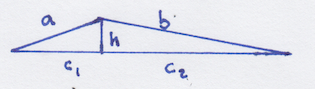
\includegraphics [scale=0.8] {T1.png} \end{center}
Then, by the Pythagorean theorem, the two parts of $c$ are clearly shorter than the sum of the two other sides since
\[ c_1^2 + h^2 = a^2, \ \ \ \ \ \ c_2^2 + h^2 = b^2 \]
Simple algebra (and a positive square root, for a length) gives $c_1 < a$ and $c_2 < b$ so 
\[ c = c_1 + c_2 < a + b \]

Euclid proves this theorem in book 1 of \emph{Elements}.  We need a preliminary theorem, called a \emph{lemma}.

$\bullet$ \ In any triangle, if one side is the longest, then the angle opposite is the greatest.

\emph{Proof}.

Given that side $AC > AB$, mark off the latter on $AC$, forming an isosceles triangle.
\begin{center} \includegraphics [scale=0.6] {greater_side.png} \end{center}
By the exterior angle theorem, $s > \angle C$.  But $\angle B > s$ (the whole is greater than any part).  It follows that $\angle B > \angle C$.

$\square$

The converse is also true:

\emph{Proof} 

Given that $\angle B > \angle C$ above.  It cannot be that $AB = AC$, because then the angles would be equal.  Suppose that $AB > AC$.  But then $\angle C > \angle B$ by the forward theorem.  But that contradicts what we're given.  Hence $AC > AB$.

$\square$

\subsection*{Triangle inequality}

In any triangle, the longest side is smaller than the sum of the two shorter sides.  Clearly, if a given side is not the longest, i.e. it is shorter than one of the others, then it must also be shorter than the sum of that other one plus the third.  For this reason, we consider only the longest side.

\emph{Proof}.

\begin{center} \includegraphics [scale=0.3] {triangle_inequality3.png} \end{center}
Given that side $AC$ is the longest in $\triangle ABC$.

Extend side $BC$ so that $BD = AB$.  By the isosceles triangle theorem, since $\triangle ABD$ is isosceles, $\angle D = \angle DAB$ (marked with magenta dots).

Then $\angle D$ is smaller than $\angle DAC$ and therefore, by the previous lemma, $AC$ is less than $DC$.  But $DC$ is equal to the sum of the two smaller sides of $\triangle ABC$.  Hence
\[ AC < AB + BC \]

$\square$

\subsection*{hypotenuse}
We said above that if one side is longer, then the angle opposite is larger.  The converse is also true but we will skip the general case.  However, we prove the specific case of a right triangle.

\emph{Proof}.

In any right triangle, the right angle is the largest angle.  The reason is that the two base angles (flanking the hypotenuse) add up to be one right angle, and they must both be non-zero.  Hence the largest must be smaller than a right angle. It follows that the hypotenuse is the longest side in a right triangle.

$\square$

\subsection*{tangent to a circle}

The simple definition of the tangent is that it touches the circle at only one point, and as a consequence, it forms a right angle there.
\begin{center} 
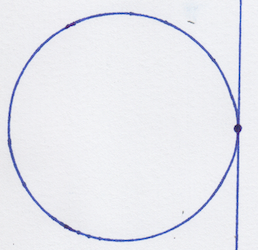
\includegraphics [scale=0.5] {T6.png} 
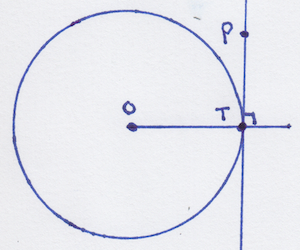
\includegraphics [scale=0.5] {T7.png} 
\end{center}

\emph{Proof}.

Suppose that the angle between the tangent and the radius at $T$ is not a right angle.  Then, there must be some \emph{other} point on the tangent line which does form a right angle when connected to the center.  There is always one such point, because we have a construction that gives the perpendicular (bisector) from a line to an external point.  

But that would make the radius to the point of tangency the hypotenuse of a right triangle.  The hypotenuse is the longest side in a right triangle, so the new point must be \emph{inside} the circle.  This is a contradiction, since the tangent touches the circle in only one point.

$\square$

Given that the tangent forms a right angle at its single point of contact, the result about the hypotenuse above (our lemma), says that any other line drawn from the center of the circle to the tangent line would be a hypotenuse and so necessarily longer than the radius to the tangent.  Such a point must be outside the circle.
\begin{center} 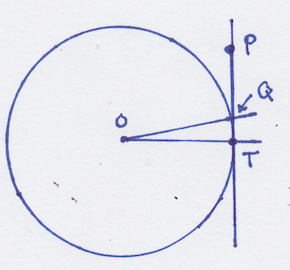
\includegraphics [scale=0.5] {T8.png} \end{center}

\end{document}
